\section{Analysis}\label{sec:analysis}

\comment{Present datasets???}

%$\datasetA = \big\{ (\vec{x}^{(1)}, y^{(1)}), \,  (\vec{x}^{(2)}, y^{(2)}), \,\dots, \, (\vec{x}^{({\npointsA})}, y^{(\npointsA)}) \big\}$ 

\comment{Maybe write something about the codes?}


OUTLINE:
\begin{enumerate}
    \item Gradient descent \begin{enumerate}
        \item[-] OLS and Ridge on regression problem
    \end{enumerate}
    \item Building our FFNN
    \item Regression problem \begin{enumerate}
        \item[-] try different activation functions
    \end{enumerate}
    \item Classification problem \begin{enumerate}
        \item[-] compare with logistic regression 
    \end{enumerate}
\end{enumerate}

\subsection{Gradient descent}

    We write a code that  \fillertext


    Using the SGD method, we perform an OLS regression on a dataset generated by a third order polynomial with some added noise,
    \begin{equation}
        f(x) = ax + bx^2 + cx^3 \, +\, d\mathcal{N}(0, 1). % fix numbers!
    \end{equation}
    In particular, we aim to minimise the cost function in eq. \eqref{eq:ols_cost_function} for which we need to tune the learning rate $\eta$. We perform the same analysis using the Ridge cost function in eq. \eqref{eq:ridge_cost_function}, but here we need to tune the penalty parameter $\lambda$ as well as the learning rate $\eta$. 

    We do not present many figures to describe this part of the analysis. We justify this by arguing that the purpose of this part is to test the SGD code, and then by extension the GD code, and give an idea of the effect of changing optimisers. 

    In Figure \ref{fig:simple_reg_errors_ols}  \fillertext

    \begin{figure}
        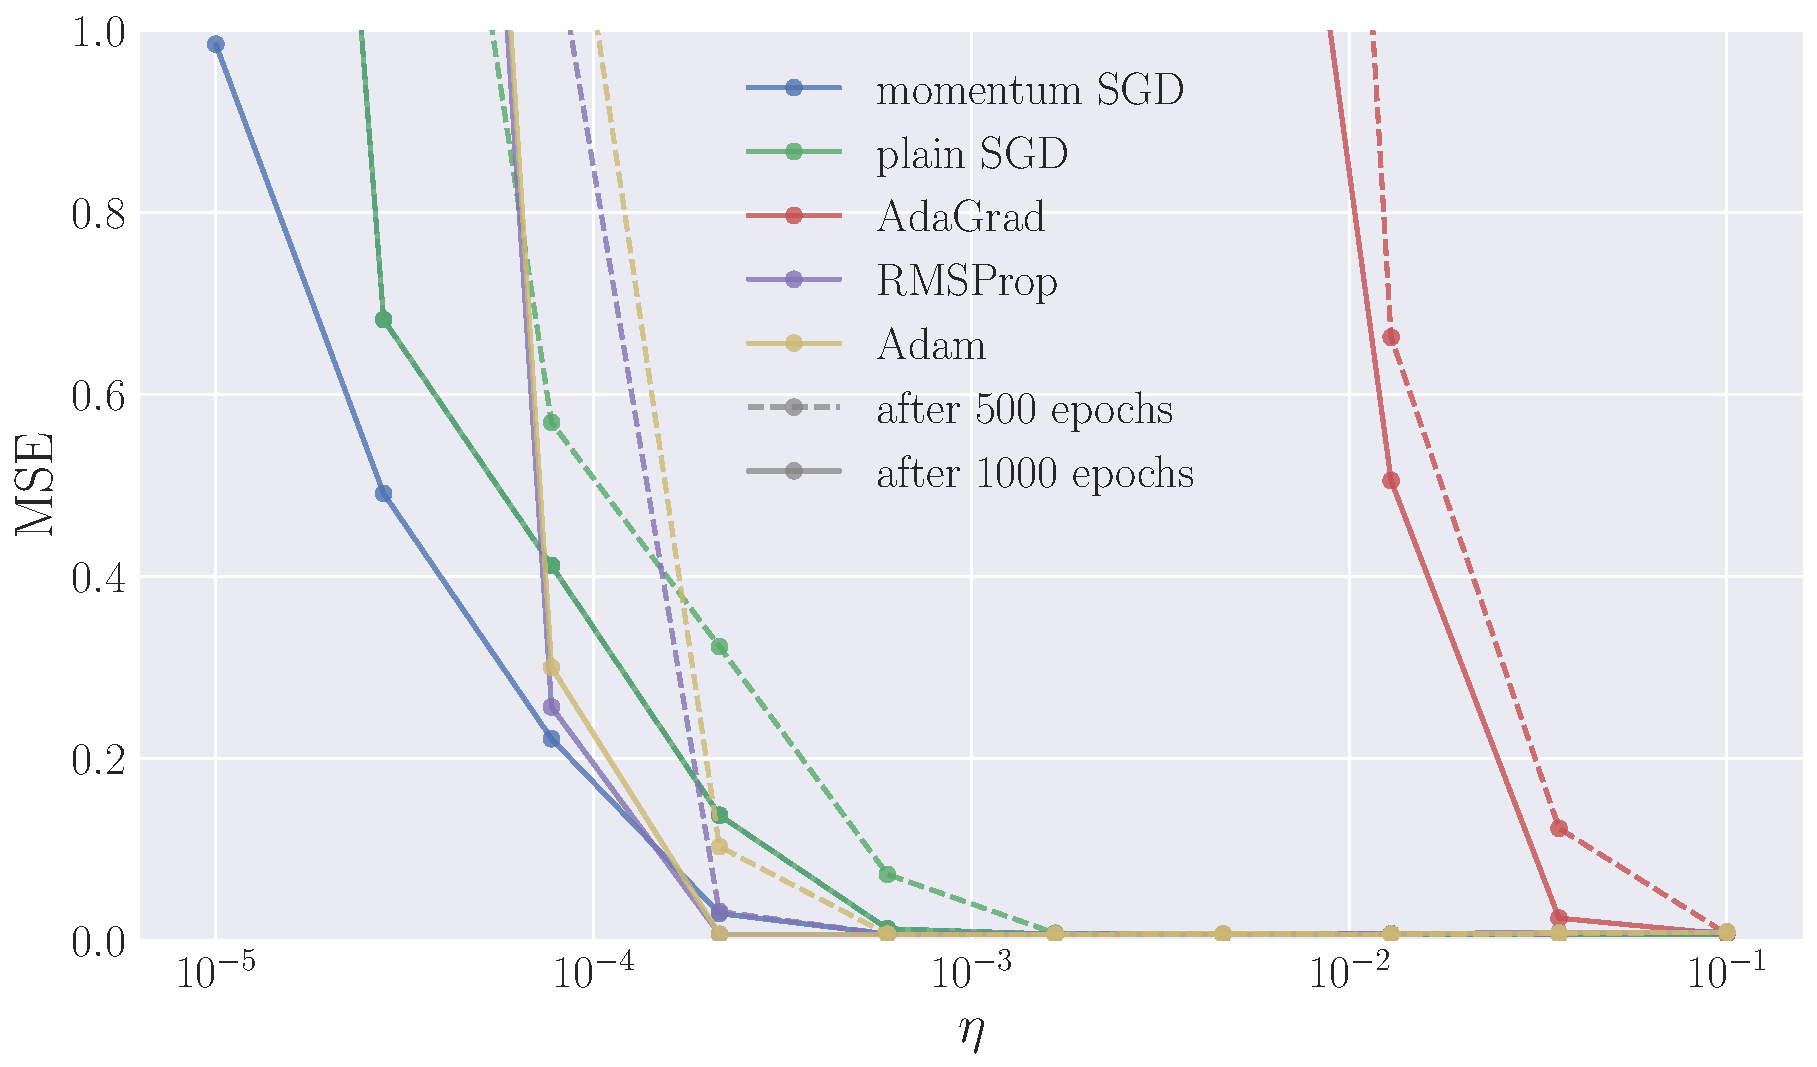
\includegraphics[width=\linewidth]{errors_gradient_descent.pdf}
        \caption{This very cute figure is ...}
        \label{fig:simple_reg_errors_ols}
    \end{figure}

    \begin{figure}
        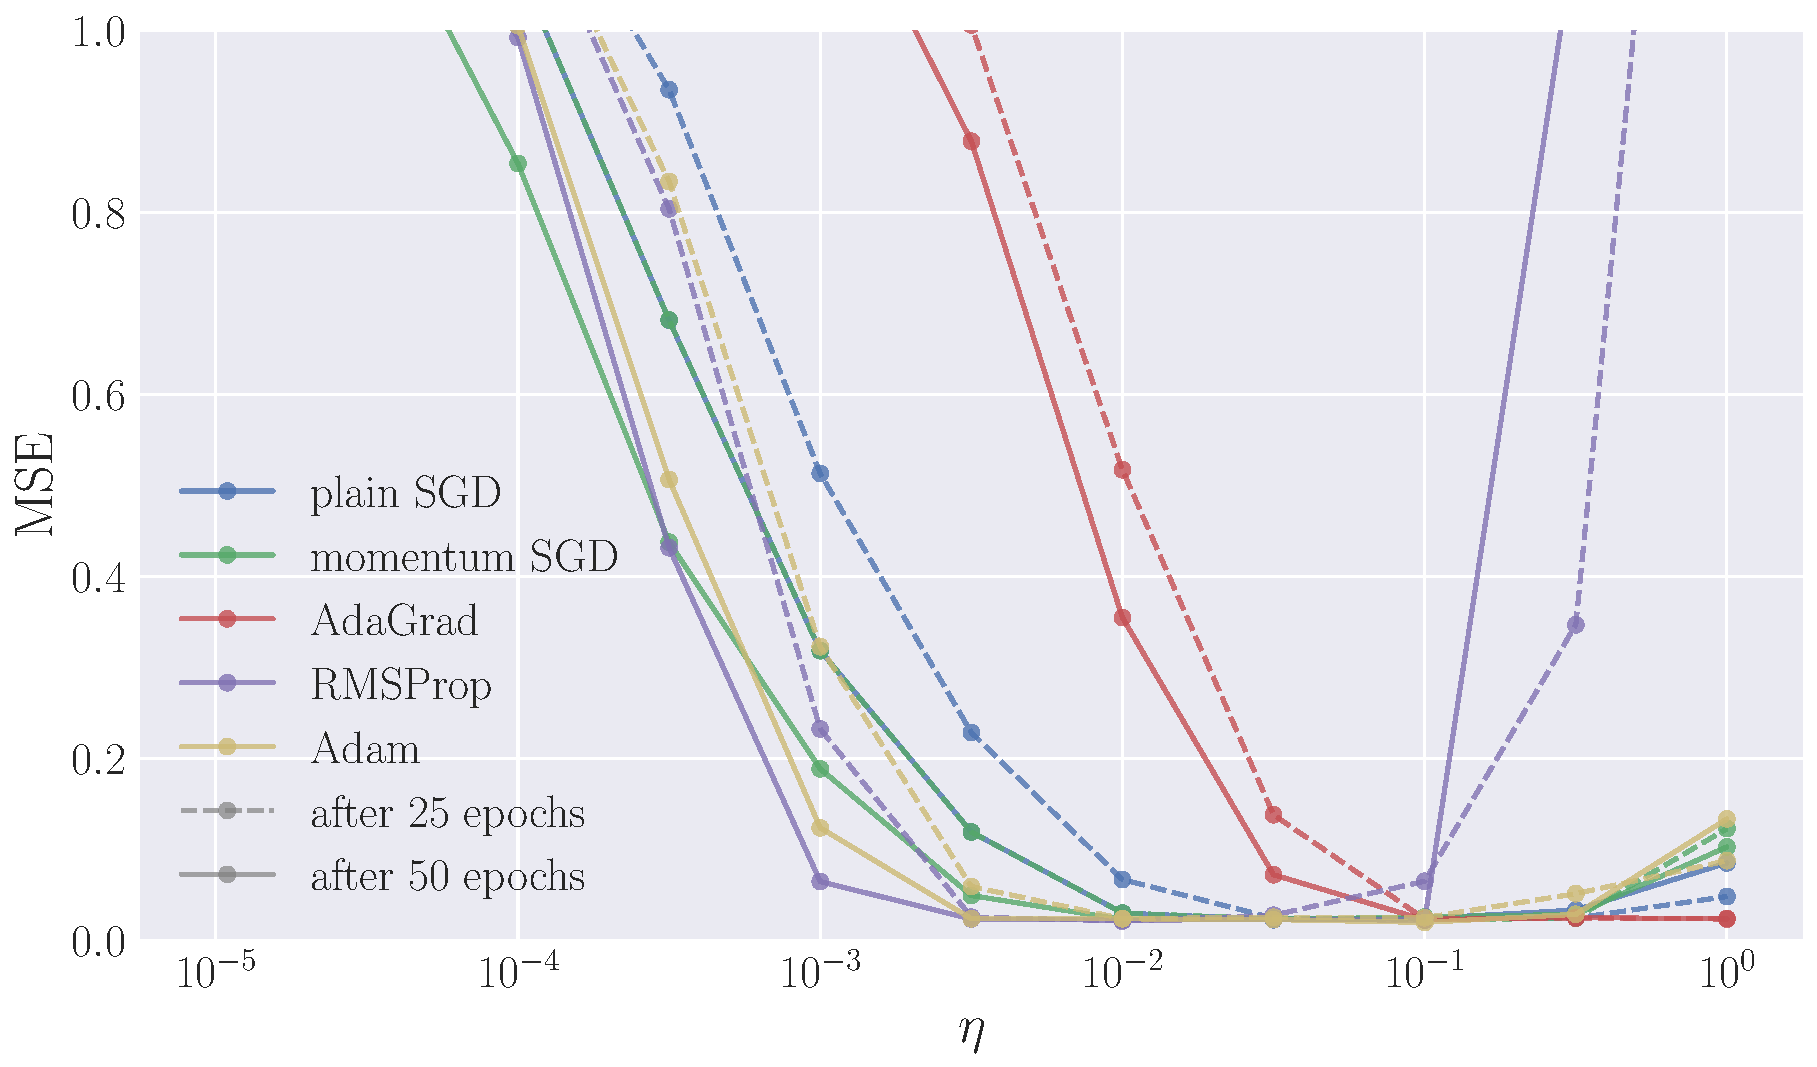
\includegraphics[width=\linewidth]{ridge_errors_gradient_descent.pdf}
        \caption{This very cute figure is \rephrase{unnecessary! Maybe remove? Or make subplot?} lambda is 0.1 i think}
        \label{fig:simple_reg_errors_ridge}
    \end{figure}




    
\subsection{Neural network}
    We will build our FFNN (\ref{item:prepocess}-\ref{item:optimiser}) and solve a supervised learning problem (\ref{item:train}-\ref{item:review}) using the steps listed below \citep{mhjensen}.

    \begin{enumerate}[label=(\roman*)]
        \item\label{item:prepocess} Collect and prepocess data, that is we extract 80\% of the dataset and reserve the rest for validation. The data is then scaled using standard score normalisation\footnote{Formula found in \cite{mhjensen}, or page 6 of the \projectOne-report.} with respect to the training data.
        \item\label{item:architecture} Define the model and design its architecture. In practice, this means to decide on hyperparameters of the NN such as depth ($L$) and activation function(s) ($g$).
        \item\label{item:optimiser} Choose loss function and optimiser. For regression we will use the regular MSE score \checkthis{(ref!)} as the estimator of loss, whereas the classification problem estimates the loss according to the accuracy score \checkthis{(ref!)}. \wtf[please send help] The choice of optimiser is between GD and SGD, but includes decisions about the exact algorithm \rephrase{(how we optimise the learning rate)}.
        \item\label{item:train} Train the network to find the right weights and biases.
        \item\label{item:assess} Validate model, i.e. assess model performance by applying it on the test data.
        \item\label{item:review} Adjust hyperparameters, and if necessary review the network architecture. That is to say, if the result is not satisfactory even after tuning the hyperparameters, return to step \ref{item:architecture} and start over from there. 
    \end{enumerate}

    %In practice, the steps \ref{item:architecture}-\ref{item:review} will be performed several times 
    

\subsection{Regression problem}\label{sec:analysis_regression}


    Our dataset is once again fictional as it is generated by the Franke function from \projectOne\footnote{Equation (10) in the report.} for a set of coordinates in the plane. We split and standardise the $20\times 20$ datapoints in accordance with step \ref{item:prepocess}. 






\subsection{Classification problem}\label{sec:analysis_classification}



